\documentclass{article}
\usepackage{tikz}
\begin{document}
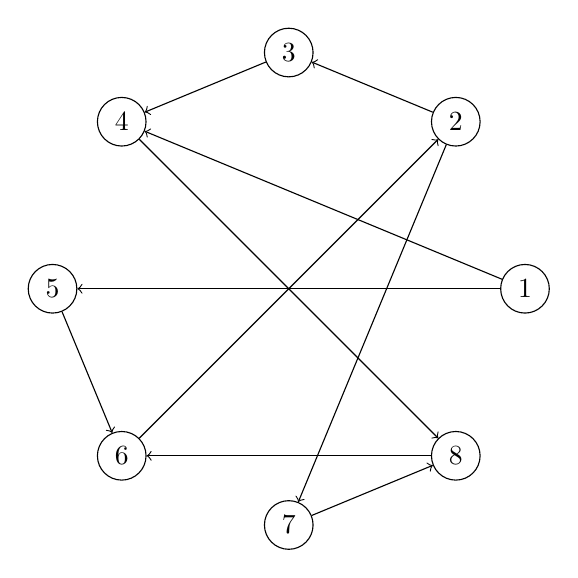
\begin{tikzpicture}[->,node distance=2cm]
\tikzstyle{every node}=[circle,draw]
\node (1) at (3.0,0.0) {1};
\node (2) at (2.121320343559643,2.1213203435596424) {2};
\node (3) at (1.8369701987210297e-16,3.0) {3};
\node (4) at (-2.1213203435596424,2.121320343559643) {4};
\node (5) at (-3.0,3.6739403974420594e-16) {5};
\node (6) at (-2.121320343559643,-2.1213203435596424) {6};
\node (7) at (-5.51091059616309e-16,-3.0) {7};
\node (8) at (2.121320343559642,-2.121320343559643) {8};
\draw[->] (1) -- (4);
\draw[->] (1) -- (5);
\draw[->] (2) -- (3);
\draw[->] (2) -- (7);
\draw[->] (3) -- (4);
\draw[->] (4) -- (8);
\draw[->] (5) -- (6);
\draw[->] (6) -- (2);
\draw[->] (7) -- (8);
\draw[->] (8) -- (6);
\end{tikzpicture}
\end{document}
